\input{~/Documents/LatexPresets/programming/preambule.tex}
%\usepackage{mathtools}
%\usepackage{amssymb}
\usepackage{hyperref}
\usepackage[perpage,bottom]{footmisc}

\newcommand{\basedir}{~/FESB/2. semestar/3D Simulacije/Izvještaji/vjezba4}
\title{Vježba L04}
\author{Jakov Spahija}

\begin{document}
\maketitle
\vspace{15em}
\tableofcontents
\pagebreak

%%%%%%%%%%%%%%%%%%%%%%%%%%%%%%%%%%%%%%%%%%%%%%%%%%%%%%%%%%%%%%%%%%%%%%%%%%%
\section{Kreiranje UWP Aplikacije}
\label{sec:UWP}
\setcounter{lstlisting}{0}

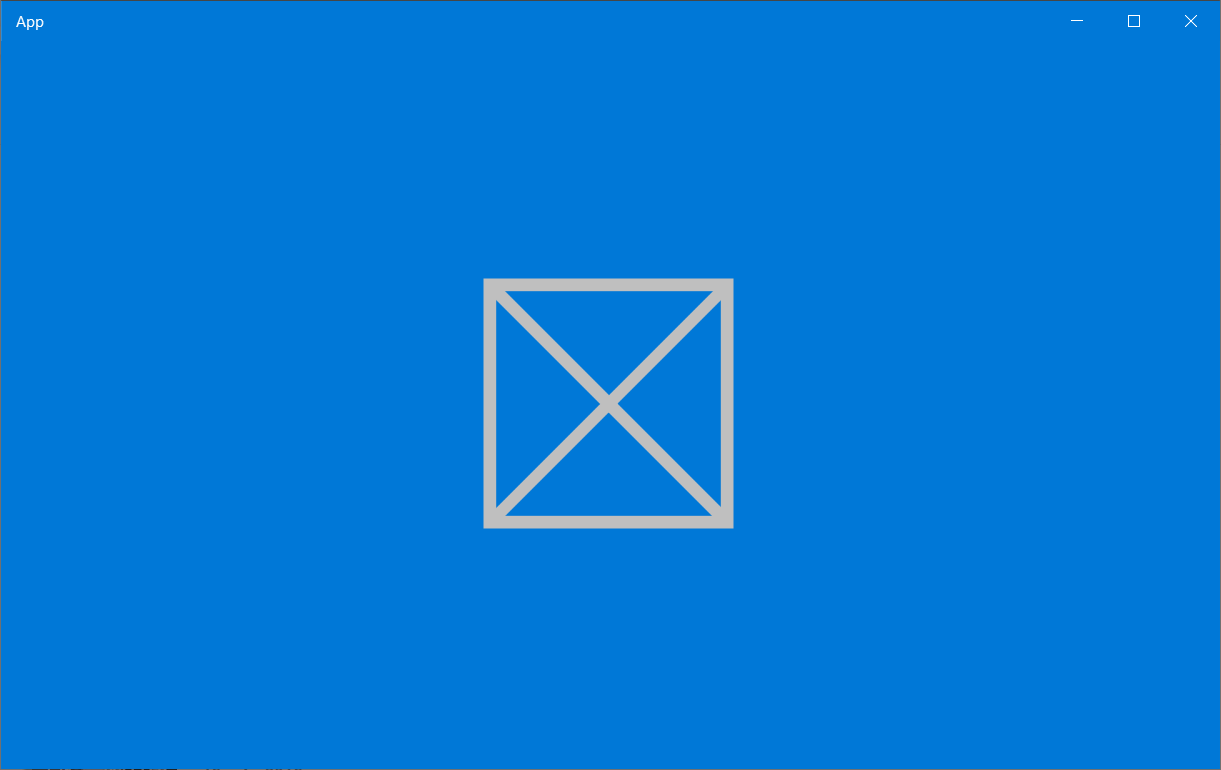
\includegraphics[width=450px]{..\\zad1\\zad1.png}

\pagebreak

%%%%%%%%%%%%%%%%%%%%%%%%%%%%%%%%%%%%%%%%%%%%%%%%%%%%%%%%%%%%%%%%%%%%%%%%%%%
\section{Životni ciklus}
\label{sec:cycle}
\setcounter{lstlisting}{0}

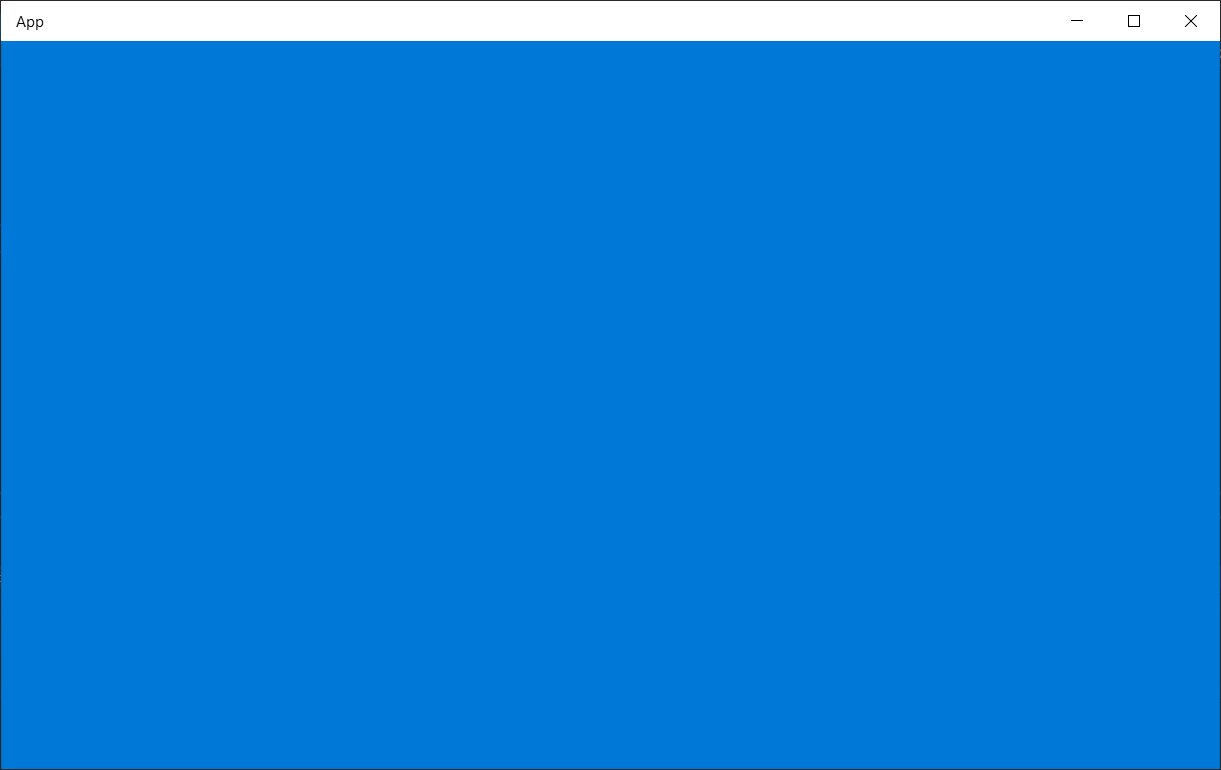
\includegraphics[width=450px]{..\\zad2\\zad2.png}

\vspace{2em}
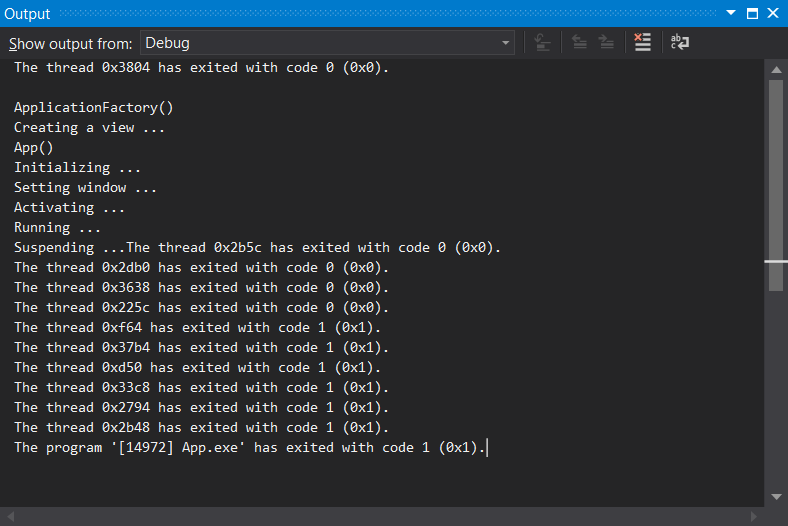
\includegraphics[width=450px]{ ..\\zad2\\debug.png }

\pagebreak

%%%%%%%%%%%%%%%%%%%%%%%%%%%%%%%%%%%%%%%%%%%%%%%%%%%%%%%%%%%%%%%%%%%%%%%%%%%
\section{Periferije: miš, tipkovnica}
\label{sec:input}
\setcounter{lstlisting}{0}

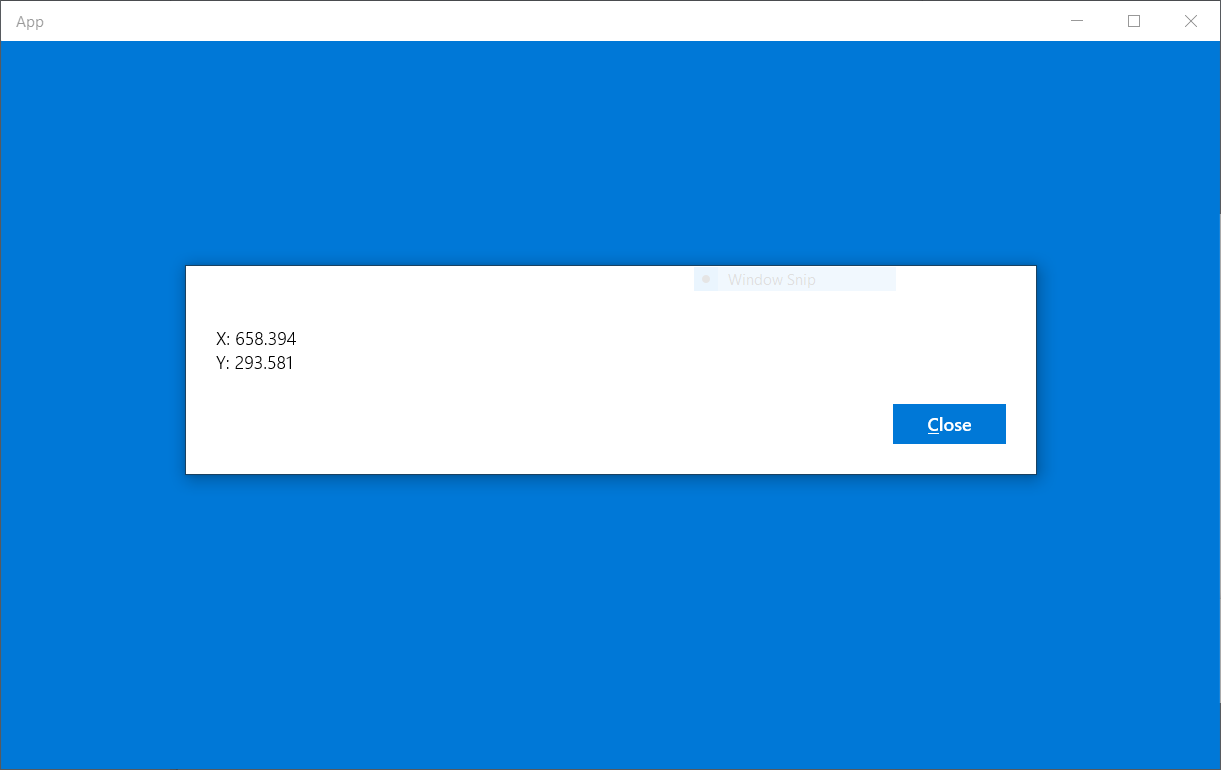
\includegraphics[width=450px]{..\\zad3\\zad3.png}

\pagebreak

%%%%%%%%%%%%%%%%%%%%%%%%%%%%%%%%%%%%%%%%%%%%%%%%%%%%%%%%%%%%%%%%%%%%%%%%%%%
\section{Brojač}
\label{sec:timer}
\setcounter{lstlisting}{0}

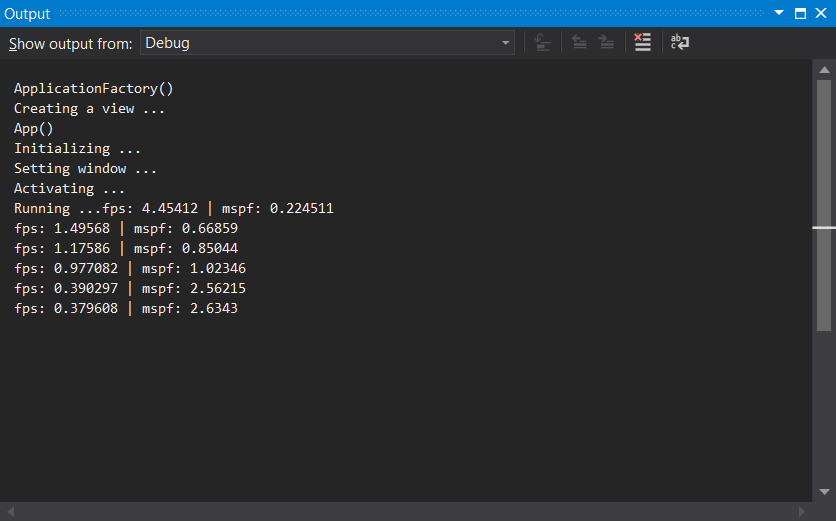
\includegraphics[width=450px]{..\\zad4\\zad4.png}

\pagebreak

\end{document}
